\documentclass[10pt,twoneside]{book}
%\documentclass[10pt,oneside]{book}
%\documentclass[14pt]{article}   	% use "amsart" instead of "article" for AMSLaTeX format
\pagestyle{headings}

\usepackage{natbib}
\usepackage{hyperref}

%\renewcommand\bibname{Bibliografía}
%\renewcommand\bibname{Bibliografy}

\usepackage{titlesec}


\usepackage{enumitem}

%\usepackage[spanish]{babel}
 
\titleformat{\chapter}[display]
  {\normalfont\bfseries}{}{0pt}{\Huge}

\usepackage{blindtext}
\usepackage[T1]{fontenc}
%\usepackage[utf8]{inputenc}

\usepackage{bbm}

\usepackage[margin=1in,footskip=.25in]{geometry}
%\usepackage[margin=1in]{geometry}
\usepackage{geometry}
\usepackage{mathtools}    
\usepackage[latin9]{inputenc}  	
\usepackage[bottom]{footmisc}	% See geometry.pdf to learn the layout options. There are lots.
\geometry{letterpaper}                   		
\usepackage{graphicx}														
\usepackage{amssymb}
\usepackage{ragged2e}
\newcommand{\kfour}{\mathbb{K}^4}
\newcommand{\ktwo}{\mathbb{K}^2}
\newcommand{\pthree}{\mathbb{P}^3}
\newcommand{\afin}{\mathbb{A}}
\newcommand{\ov}{\overrightarrow}


\usepackage{tikz-cd}


\usepackage{faktor}


\usepackage{mathtools}


%\usepackage[spanish]{babel} % español
%\usepackage[utf8]{inputenc} % acentos sin codigo
%\usepackage{graphicx} % graficos
%\usepackage{amssymb} 
%\usepackage{amsmath,amsthm} 
%\usepackage{amsthm} 

%\usepackage{hyperref}
%\usepackage{mathtools}
\usepackage{mathrsfs} % Letras caligráficas
\usepackage{bm}


\usepackage{tikz-cd}
\usepackage{xcolor}

\newcommand{\mcm}{\qopname \relax o{mcm}}

\newcommand{\massey}[3]{\langle[ {#1} ],[ {#2} ],[ {#3} ]\rangle}
\newcommand{\module}[1]{\vert #1 \lvert }
\newcommand{\dotprod}[2]{\langle #1,#2 \rangle}
\newcommand{\mbot}{{(\bot)}}
%\newcommand{\isoequal}{\stackrel{\text{iso}}{=}}
\newcommand{\isoequal}{\simeq}
\newcommand{\difequal}{\stackrel{\text{dif}}{=}}
\newcommand{\defequal}{\stackrel{\text{def}}{=}}
\newcommand{\isoapprox}{\stackrel{\text{iso}}{\displaystyle\approx}}
\newcommand{\Cech}{\v{C}ech}
\newcommand{\difpartial}[2]{\frac{\partial #1}{\partial #2}}
\newcommand{\difantipartial}[2]{\frac{\partial #1}{\overline{\partial} #2}}
\newcommand{\antipartial}{{\overline{\partial }}}

\newcommand{\comilla}{{}"{}}


\newcommand{\e}[2]{e_{#1}^{(#2)}}

\newcommand{\f}[2]{f_{#1}^{(#2)}}


\usepackage{amsthm}

\newcounter{fakecnt}[section]
\def\thefakecnt{\arabic{section}}

\newtheorem{theorem}{Theorem}
\newtheorem*{notation}{Notation}
\newtheorem{proposition}{Proposition}
\newtheorem*{conjecture}{Conjecture}
\newtheorem{remark}{Remark}
\newtheorem{corollary}{Corollary}[theorem]
\newtheorem{lemma}{Lemma}[chapter]
\newtheorem{observation}{Observation}[chapter]
\newtheorem{example}{Example}[chapter]
%\renewcommand{proof}{\prof}
\theoremstyle{definition}
	\newtheorem{definition}{Definition}[chapter]
	

\newenvironment{hproof}{%
  \renewcommand{\proofname}{Esquema de demostraci�n}\proof}{\endproof}
  
 \newenvironment{prof}{%
  \renewcommand{\proofname}{Proof}\proof}{\endproof}


\newcommand{\ifff}{if and only if }


\renewcommand\qedsymbol{$QED$}


%\footskip = 0pt

\graphicspath{ {imgs/} }

\date{}
\begin{document}
%\autor{Mario Marhuenda Beltrán}

%\tableofcontents

\flushleft

\newcommand{\R}{\mathbb{R}}
\chapter{Morse theory: A quick review}
\begin{notation}

We will consider all complexes to be over a field
$\mathbb{K}$ that will either be 
 $\mathbb{Q}$,
 $\mathbb{R}$,
 or 
  $\mathbb{C}$.
Unless otherwise stated.
\end{notation}


\begin{definition}[Differential complex]
We say that a collection of indexed abelian groups
$\{C_i\}_{i=0}^{\infty}$ is a differential complex if
it has a linear operator:
$\delta_i: C_{i+1}\to C_i$
so that $\delta_i\circ\delta_{i+1}=0$.

Usually, we shall consider $\delta: C\to C$ where $C=\oplus C_i$
and $\delta$ is defined as the unique linear operator that coincides with $\delta_i$
when the domain is restricted to $C_i$.

And so, we may write that $\{C_i\}_{i=0}^{\infty}$ 
is a differential complex if and only if $\delta^2=0$.
\end{definition}

Given a manifold we can build a nice function on it, $f$,
so that it's sublevels $M^t=f^{-1}(-\infty,t]$ give us a natural way to 
deduce a CW-structure for the manifold.

In fact, these same function give us in a natural way the Morse-Smale complex,
which allows us to compute the homology of the manifold.

\begin{definition}[Morse function]

Let $M$ be a manifold, and $f\in C^\infty(M,\mathbb{R})$.
We say that $f$ is a morse function if the set of critical points
of $f$ is isolated. 

That is, if:
$
Crit(f)=\{x\in M: df\vert_x=0
\}
$
is isolated.

\end{definition}

We say that a critical point of $f$ has index $k$,
if the hessian of $f$ has index $k$ at the critical point.

We denote the critical points of index $k$ as $Crit_k(f)$.

It is well known that for any given manifold there are plenty of Morse functions,
in particular we have the following:


\begin{theorem}
\cite{mat1997}
Let $g\in C^\infty(M,\mathbb{R})$, and let $\epsilon>0$
then there exists $f\in C^\infty(M,\mathbb{R})$ so that $f$
is a Morse function and $f$ and $g$ are $C^2$-close.
\end{theorem}

So Morse functions are dense in the ring $C^\infty(M,\mathbb{R})$,
and a fortiori, Morse functions always exits.

Morse functions give quite a bit of topological information on the manifold,
specially in the compact case. 



One important source of complexes is the Morse-Smale complex,
which arises in a natural way.


\section{Fundamental theorems of Morse theory}

\begin{theorem}[Morse lemma]
\cite{mat1997}
Let $M^n$ be a manifold, and $f$ a Morse function on $M$.
Let $x_0$ be critical point of $f$ of index $k$.


Then there is a neighbourhood $V$ of $x_0$ and a chart 
$y:U\to V\subset M$. so that:

$$
f\circ y (y_1,\ldots,y_n)
=
-y_1^2
-\cdots
-y_k^2
+y_{k+1}^2
+\cdots
+y_n^2
+C
$$

Where $C$ is a constant.
\end{theorem}

Let $f$ be a Morse function on $M$,
We notice that in the compact case $f$ has 
a minimum, $m$ and a maximum $M$
achieved at points $x_m$ and $x_M$.

Then $M^{x_m}=\emptyset$ and $M^{x_M}=M$.
This hints that we can restruct $M$ from how the sets $M^t$
change as $t$ moves through the real line.

In particular, fix some $\varepsilon$ which will be assumed to be
as small as needed, we wonder if there is any relation between $M^t$
and $M^{t+\varepsilon}$. It turns out, as Morse \cite{mor1934} showed
we have that if $f$ does not have any critical point in the interval 
$(t,t+\varepsilon)$ then
 $M^t$ and $M^{t+\varepsilon}$ are difeomorphic. The proof is
 in fact quite elementary.
 
 A more subtle thing Morse proved is what happens when $M^t$
 crosses over a critical point. In this cased he showed that,
 if choose $\varepsilon$ so that $Crit(f)\cap (t,t+\varepsilon)$
 has exactly one point (which we can always do by hypothesis)
 then
  $M^{t+\varepsilon}$ can be obtained by adjoining a $k$-cell to $M^t$
 where $k$ happens to be the index of the unique critical point in 
$(t,t+\varepsilon)$.


In summary

\begin{theorem}
\cite{mor1934}
Let $\varepsilon>0$ so that
$$Crit(f)\cap (t,t+\varepsilon)=\emptyset$$

Then   $M^{t}$ and $M^{t+\varepsilon}$ 
are difeomorphic.


\end{theorem}

\begin{theorem}
\cite{mor1934}
Let $\varepsilon>0$ so that
$$Crit(f)\cap (t,t+\varepsilon)=\{x_0\}$$

Let $k$ be the index of $x_0$. Then

Then  $M^{t+\varepsilon}$ 
is homotopy equivalent to $M^t\cup_\phi (D^{n-k}\times D^k)$ where
$D^k$ is the $k$-disk and $\phi$ is and adjunction map
between $\partial (D^{n-k}\times D^k)$ and $\partial M^t$.


\end{theorem}


\begin{corollary}
\cite{sma1961}
Any compact manifold 
of dimension $n$
is homotopy equivalent to a space such as the following:

$$
D^n\cup
D^{n-k_1}\times D^{k_1}
\cup
\cdots
\cup
D^{n-k_m}\times D^{k_m}
$$
\end{corollary}


\begin{theorem}[Morse inequalities]
Let $M$ be a compact manifold, and $b_i$ it's betti numbers.
Let $f$ be a Morse function on $M$. And let $\lambda_k$ be the 
number of $k$-index critical points of $f$. Then we have that:

$$
\lambda_i\geq b_i,\quad
\forall i\in\mathbb{N}
$$

\end{theorem}

\section{An application of Morse theory}

In this section we describe how to use Morse theory to classify closed $1$-manifolds.
In particular, we show the well-know theorem:

\begin{theorem}
A closed connected $1$-manifold is diffeomorphic to $\mathbb{S}^1$.
\end{theorem}

We briefly mention that it can be used to derive the usual classification of $2$-manifolds.





\section{The Morse-Smale complex}

Morse functions give a natural complex which computes the homology
of the manifold.

We define the chain groups 
to be:

$$
C_f(f)
\defequal
\left\{
\sum
_
{c\in Crit_k(f)}
a c
\vert
a\in \mathbb{Z}_2
\right\}
$$

And we define the differential operator $\partial$ to be:

$$
\partial a
=
\sum
_{b\in Crit_k(f)}
n(a,b)b
$$

Where $n(a,b)$ is the number of trajectories flowing from $a$
to $b$ through the gradient flow. This number is finite, and
we have that $\partial^2=0$.




\chapter{Elder-rule Staircodes}

\chapter{Morse functions on point clouds}

We now focus on discrete augmented metric spaces.
In particular, suppose we have a compact smooth manifold
$M$ equipped with a Morse function $f:M\to \mathbb{R}$.

From this manifold $M$ we sample a finite amount of points 
$X=\{x_i\}_{i=0}^n$ and we record the value of $f$ on $X$.

We investigate what sort of topological information we can recover from this
discrete sample.

The first thing we would like to do is recover the gradient of the function.
For this purpose we create a graph using $X$ as its base set
and we define a flow on the graph by moving from one point to the point
connected with it where the morse function $f$ takes the smallest value.

\begin{definition}[NNG graph]

Given $X$ a discrete set,
we define $G^-(X)$ it's descending pseudo-gradient graph
as the nearest neighbour graph of $X$. 

That is the graph where the 
edges $\{x_i,x_j\}$ are precisely where either $d(x_i,x_j)=d(x_i,X)$
or $d(x_i,x_j)=d(x_j,X)$. Notice that the binary relation $x_i\sim x_j$ if 
and only if
$x_j$ is the closest vertex to $x_i$ is not symmetric.

We denote as $\omega^-:G\to G$ the application that
maps $p\in X$ to the result of iteratively following the point
with that its joined to $p$ and that minimises the value of $f$.

We define $\alpha^-$ in an analogous manner, by following the direction 
of maximum growth of $f$.
\end{definition}

\begin{example}
For example, let's consider the following graph, where we denote the
value of $f$ by $x_i:f(x_i)$:

%\begin{center}
%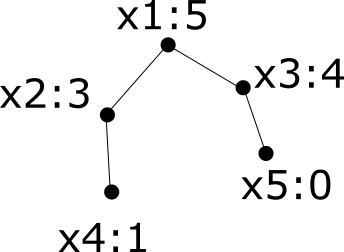
\includegraphics[height=3cm]{nng1.png}
%\end{center}

\begin{center}
%\begin{tikzpicture}
%[scale=.8]
%%\node[parameters] (nodeID) {nodeLabel};
%%  [scale=.8,auto=left,every node/.style={circle,fill=blue!20}]
%%  \node (n6) at (1,10) {6};
%%  \node (n4) at (4,8)  {4};
%%  \node (n5) at (8,9)  {5};
%%  \node (n1) at (11,8) {1};
%%  \node (n2) at (9,6)  {2};
%%  \node (n3) at (5,5)  {3};
%\node[main] (1) [above of=2] {$x_1$}
%\node[main] (2) [below left of=1] {$x_2$}
%\node[main] (3) [below right=1] {$x_3$}
%
%
%%  \foreach \from/\to in {n6/n4,n4/n5,n5/n1,n1/n2,n2/n5,n2/n3,n3/n4}
%%    \draw (\from) -- (\to);
%
%\end{tikzpicture}


\begin{tikzpicture}[node distance={30mm}, thick, main/.style = {draw, circle}] 
\node[main] (1) {$x_1\mapsto 5$}; 
\node[main] (2) [below left of=1] {$x_2\mapsto 3$}; 
\node[main] (3) [below right of=1] {$x_3\mapsto 4$}; 
\node[main] (4) [below of=2] {$x_4\mapsto 1$}; 
\node[main] (5) [below left of=3] {$x_5\mapsto 0$}; 
\node[main] (6) [below right of=3] {$x_6\mapsto 3$}; 
\draw (1) -- (2); 
\draw (1) -- (3); 
\draw (2) -- (4); 
\draw (3) -- (5); 
\draw (3) -- (6); 
\end{tikzpicture} 

\end{center}

Then $\omega^-(x_1)=x_4$. So $\omega$ maps 
to local minimums, but not necessarily to absolute ones,
even when restricting to the same component. 


\end{example}





\bibliographystyle{plain}

\bibliography{tfm}

\end{document}
